%% LaTeX2e class for seminar theses
%% seminar.tex
%% 
%% Karlsruhe Institute of Technology
%% Institute for Program Structures and Data Organization
%% Chair for Software Design and Quality (SDQ)
%%
%% Dr.-Ing. Erik Burger
%% burger@kit.edu
%%
%% Version 1.0.4, 2021-06-21

%% Available page modes: oneside, twoside
%% Available languages: english, ngerman
%% Available modes: draft, final (see README)
\documentclass[twoside, ngerman]{sdqseminar}

%% ---------------------------------
%% | Information about the thesis  |
%% ---------------------------------

%% Name of the author
\author{Alina Valta}

%% Title (and possibly subtitle) of the thesis
\title{Refaktorisierung einer Architekturanalyse für Vertraulichkeit}

%% Type of the thesis 
% \thesistype{Seminar Thesis}

%% Change the institute here, ``KASTEL'' is default
% \myinstitute{Institute for \dots}

%% The advisors are PhD Students or Postdocs
\advisor{M.Sc. Frederik Reiche}

\settitle

%% --------------------------------
%% | Settings for word separation |
%% --------------------------------

%% Describe separation hints here.
%% For more details, see 
%% http://en.wikibooks.org/wiki/LaTeX/Text_Formatting#Hyphenation
\hyphenation{
% me-ta-mo-del
}

%% --------------------------------
%% | Bibliography                 |
%% --------------------------------

%% Use biber instead of BibTeX, see README
\usepackage[citestyle=numeric,style=numeric,backend=biber]{biblatex}

\usepackage{listings}
\usepackage{svg}
\addbibresource{seminar.bib}

%% ====================================
%% ====================================
%% ||                                ||
%% || Beginning of the main document ||
%% ||                                ||
%% ====================================
%% ====================================
\begin{document}

%% Set PDF metadata
\setpdf

%% Set the title
\maketitle

%% ----------------
%% |   Abstract   |
%% ----------------
 
%% The text is included from the following files:
%% - sections/abstract

\begin{abstract}
%\input{sections/abstract.tex}
\end{abstract}

%% -----------------
%% |   Main part   |
%% -----------------


%\input{sections/introduction.tex}
%%% LaTeX2e class for seminar theses
%% sections/content.tex
%% 
%% Karlsruhe Institute of Technology
%% Institute for Program Structures and Data Organization
%% Chair for Software Design and Quality (SDQ)
%%
%% Dr.-Ing. Erik Burger
%% burger@kit.edu

\section{First Content Section}
\label{ch:FirstContentSection}

%% -------------------
%% | Example content |
%% -------------------
The content chapters of your thesis should of course be renamed. How many
chapters you need to write depends on your thesis and cannot be said in general.

Check out the examples theses in the SDQWiki:

\url{https://sdqweb.ipd.kit.edu/wiki/Form_der_Ausarbeitung_bei_Seminaren}

Of course, you can split this .tex file into several files if you prefer. 


\subsection{First Subsection}
\label{sec:FirstContentSection:FirstSubSection}

\dots

\subsection{A Subsection}
\label{sec:FirstContentSection:FirstSubSubSection}

\dots


\section{Second Content Section}
\label{ch:SecondContentSection}

\dots

\subsection{First Subsection}
\label{sec:SecondContentSection:FirstSubsection}

\dots

\subsection{Second Subsection}
\label{sec:SecondContentSection:SecondSubsection}

\dots

Add additional content sections if required by adding new .tex files in the
\code{sections/} directory and adding an appropriate 
\code{\textbackslash input} statement in \code{thesis.tex}. 
%% ---------------------
%% | / Example content |
%% ---------------------
%\input{sections/conclusion.tex}


\section{Aufgabenstellung}
Die Aufgabe dieses Praktikums ist eine Refaktorisierung der Projekte Confidentiality4CBSE\cite{Confidentiality4CBSE} und PCM2Prolog\cite{PCM2Prolog}. Die Aufgabe besteht dabei aus zwei Teilen: Die Entfernung des Profil-Mechanismus aus dem Confidentiality4CBSE Projekt und dem Verfeinern des Modells, sodass der Informationsfluss genauer modelliert werden kann. Außerdem soll es sich bei dem Praktikum um eine Refaktorisierung handeln, weshalb der PCM2Prolog Generator so angepasst werden muss, dass trotz verändertem Modell die Ausgabe als Prolog Prädikate unverändert bleibt.

\section{Setup}
Um das Projekt Confidentiality4CBSE in Betrieb zu nehmen, müssen folgende Projekte und Submodule richtig in Ecplise eingebunden werden:
\begin{itemize}
	\item Installation desEclipse Modeling Tools\footnote{https://www.eclipse.org/downloads/packages/release/2020-12/r/eclipse-modeling-tools} (Version 2020-12)
	\item Installationen über den „Install new Software…“ Dialog von Eclipse:
	\begin{itemize}
		\item Palladio Component Model\footnote{https://updatesite.palladio-simulator.com/palladio-bench-product/releases/4.3.0/} (Version 4.3)
		\item SDQ Commons\footnote{https://kit-sdq.github.io/updatesite/release/commons/} (EMF Commons und MDSD Profiles Commons)
	\end{itemize} 
	\item Clonen folgender Projekte von GitHub (inklusive aller Submodule) und Import in Eclipse:
	\begin{itemize}
		\item Confidentiality4CBSE\footnote{https://github.com/KASTEL-SCBS/Confidentiality4CBSE.git}
		\item PCM2Prolog\footnote{https://github.com/KASTEL-SCBS/PCM2Prolog.git}
	\end{itemize}
\end{itemize}
Um die Vertraulichkeitsanalyse durchzuführen, wird das Modul \code{confidentialitymm} als Eclipse Application ausgeführt. In der inneren Eclipseinstanz können eigene Projekte erstellt werden oder eines Beispiel Projekte\footnote{https://github.com/KASTEL-SCBS/Examples4SCBS} importiert werden. Jetzt können die Dateien, die in in der Analyse berücksichtigt werden sollen markiert werden. Dann kann über Rechtsklick auf \code{Create Prolog XSB Code} die Generierung des Prolog Code gestartet werden. Das Ergebnis befindet sich dann im den \code{.P} Dateien des \code{src-gen} Ordner.

\section{Vertraulichkeitsanalyse}
Die Idee hinter der Vertraulichkeitsanalyse für die Komponenten basierte Softwareentwicklung ist in dem technischen Bericht\cite{kramer2017model} von Max Kramer beschrieben worden. Es geht dabei darum eine Analyse über die Vertraulichkeit des Systems auf Architekturebene durchzuführen.

Die Architektur des Systems wird im Palladio Komponenten Modell spezifiziert. Auf dieser Basis können dann, mit Hilfe des Confidentiality4CBSE Projekts, Vertraulichkeitsinformationen ergänzt werden. Durch den UML Profil-Mechanismus können bestehende Palladio Komponenten mit Stereotypen annotiert werden, die Informationen über die Vertraulichkeit von Informationsflüssen an Interfaces oder von Operationen angeben oder Eigenschaften von Ressourcen spezifizieren. Dabei kann es sich zum Beispiel um Maßnahmen zum Schutz von Server vor Angreifern handeln oder um Information welche Daten unverschlüsselt übertragen werden. Das Profil referenziert dabei Klassen aus dem Confidentiality-Modell. Dieses Modell definiert Schutzmechanismen, Angreifer und Datenset, die für die Architektur relevant sind.

Die Analyse erfolgt in zwei Schritten: Zuerst werden die modellierten Vertraulichkeitsinformationen in Prolog Prädikate übersetzt. Dies wird von dem Projekt PCM2Prolog umgesetzt. Danach werden die Prolog Prädikate analysiert und wenn es ein Problem gefunden wird, wird dieses textuell ausgeben. In diesem Praktikum sind jedoch nur die Schritte bis zu den Prolog Prädikaten relevant.

\section{Modell}
Das Modell besteht aus fünf Paketen: \model{Data}, \model{Repository}, \model{System}, \model{Resources} und  \model{Adversary}. Diese Aufteilung wurde in der Refaktorisierung beibehalten. Die Funktionalität des Profils wird in dem neuen Modell den Paketen \model{Repository} und \model{Resources} hinzugefügt. Um den Profil-Mechanismus des Modells zu entfernen, mussten neue Klassen eingeführt werden, welche wiederum Referenzen auf Palladio Komponenten haben. 
\subsection{Data}
Das Paket \model{Data}, zusehen in \autoref{dataPackage}, wird dazu verwendet Ein- und Ausgabedaten von Komponenten in einzelne Datensätze \model{DataSets} gruppieren. Die Trennung in einzelne \model{DataSets} könnte beispielsweise nach Benutzergruppen oder Zweck der Daten erfolgen. Als \model{InformationFlow} modellierte Datenflüsse ordnen die Ein- und Ausgabedaten der Komponenten dann diesen \model{DataSets} zu. Außerdem gib es die Möglichkeit eine Gruppe von Datensätze zu definieren: Eine \model{DataSetMap}. Diese kann zum einen dafür genutzt werden, um \model{DataSets} für verschiedene Zugriffsrechte zu definieren. Für jedes Zugriffsrecht wird ein \model{SpecificationParameter} definiert und für eine \model{DataSetMap} gibt es mehrere Datensätze (\model{ParamiziedDataSetMapEntry}) mit einem jeweils zugewiesenem Zugriffsrecht. Zum anderen kann ein Datensatz auch für verschiedene User definiert werden, wenn modelliert werden soll, dass mehrere User das System verwenden und diese nur teilweise die Daten des Anderen kennen dürfen. Dazu kann für ein Datensatz und einen User ein \model{DataSetMapEnty} erstellt werden.

Im ursprünglichen Modell hattet ein \model{DataSetMapEntry} kein eigenen Parameter, um den User zu identifizieren, sondern der Name des \model{DataSetMapEntry} wurde als Attributwert angegeben, wenn dieser User referenziert werden soll. Um diese Referenz explizit zu machen, wurde im neuen Modell die Klasse \model{UserIdentifier} hinzugefügt.

\begin{figure}[htbp]
	
	\centering
	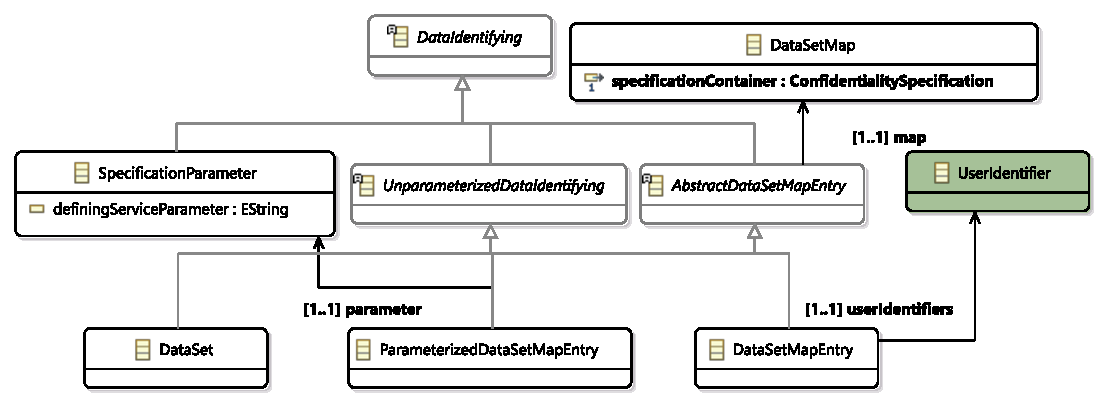
\includegraphics[width=\textwidth]{images/new/data.pdf}
	\caption{Klassendiagramm des Pakets \model{Data} mit neuer Klasse \model{UserIdentifier}, um Referenzen auf die User, die zu dem \model{DataSetMapEntry} gehören, zu ermöglichen.}\label{dataPackage}
\end{figure}
\subsection{System}
Im Paket \model{System}, zusehen in \autoref{fig:systemPackage}, wurde in der Klasse \model{DataSetMapParameter2"-KeyAssignment} das Attribute \model{assigendKey} von einem String Attribut zu einer Referenz zu \model{UserIdentifier} geändert \ref{fig:systemPackage}. Im bisherigen Modell wurde hier der Name eines \model{DataSetMapEntry} eingetragen. Durch diese Änderung wird die Beziehung zwischen einem \model{DataSetMapEntry} und der Klasse \model{DataSetMapParameter2KeyAssignment} explizit modelliert. Diese Klasse modelliert, dass ein \model{Connector} ein User authentifiziert und ihm ein bestimmtes Zugriffsrecht (\model{SpecificationParameter}) zuweist. Die Stereotypen \model{InformationFlowParameterEquation} und \model{InformationFlowParameterAssignment}\ref{systemProfil} des Confidentiality-Profils, zusehen in \autoref{systemProfil}, wurden entfernt, indem den Klassen \model{SpecificationParameterEquation} und \model{AbstractSpecifiationParameterAssignment} jeweils eine Referenz zu einem oder mehreren \model{AssemblyContexten} beziehungsweise \model{Connectoren} hinzugefügt wurde.
\begin{figure}
	\centering
	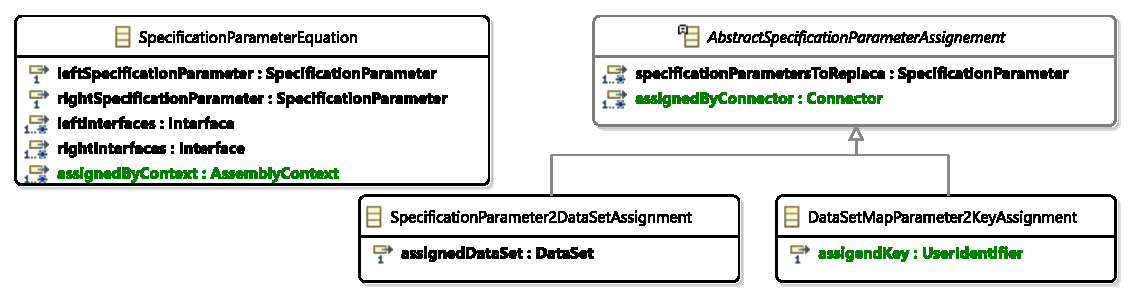
\includegraphics[width=\textwidth]{images/new/system.pdf}
	\caption{Klassendiagramm des Pakets \model{System}. Die grün markierten Referenzen wurden hinzugefügt, um die Stereotypen  \model{InformationFlowParameterEquation} und \model{InformationFlowParameterAssignment} (siehe Abb. \ref{systemProfil}) zu ersetzen.}\label{fig:systemPackage}
\end{figure}
\begin{figure}[htbp]
	\centering
	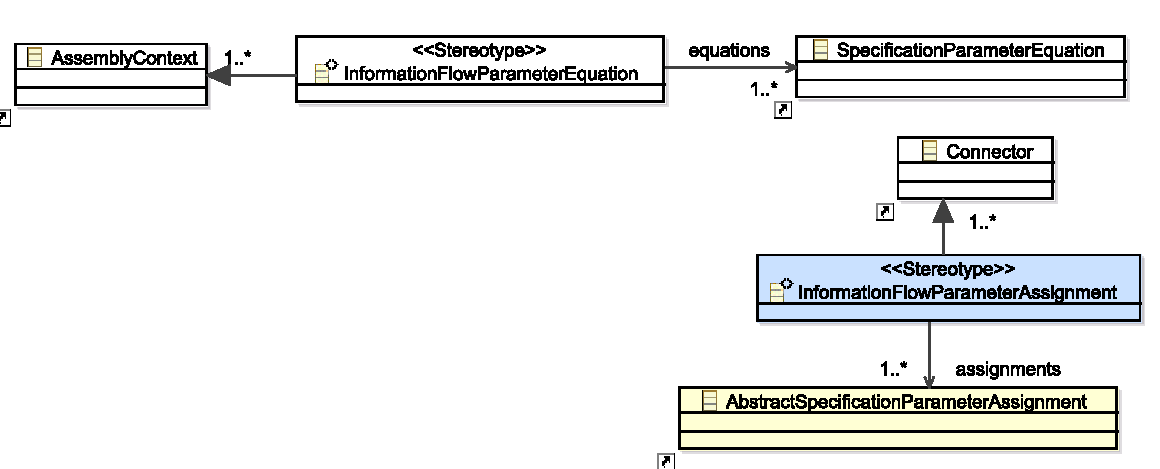
\includegraphics[width=\textwidth]{images/old/systemProfile.pdf}
	\caption{Teil des Confidentiality-Profils, welcher durch neue Referenzen im Paket \model{System} ersetzt wurde.}\label{systemProfil}
\end{figure}

\subsection{Repository}
Das Paket \model{Repository} ist in \autoref{repositoryPackage} zu sehen.
Der \model{InformationFlow} Stereotyp weist Interfaces oder Signaturen \model{ParameterAndDataPairs} zu. Diese wiederum weisen ein oder mehrere \model{DataSets} bestimmte Ein- oder Ausgabedaten dieser Schnittstellen oder Methoden zu, indem das String Attribut \model{parameterSources} entweder der Name eines Parameter oder ''$\backslash$call'', ''$\backslash$return'', ''*'' (alle Information) oder ''sizeof(<parameterSourceString>)'' ist. Diese Modellierung ist uneindeutig, wenn mehrere Parameter den selben Namen haben. Außerdem muss der Syntax bekannt sein. Deshalb wurde im neuen Modell ein weiteres Paket \model{Information} (siehe \autoref{informationPackage}) eingeführt, das die \model{ParameterAndDataPair} Klasse ersetzen soll. Die abstrakte Klasse \model{Information} repräsentiert hierbei ein \model{ParameterAndDataPair} welches jedoch nur noch eine \model{parameterSource} haben kann. Diese Einschränkung wurde vorgenommen, da so die Unterklassen direkt den Wert des String Attributes ersetzen können. Zum Beispiel ersetzt die Klasse \model{CallInfomation} ein \model{ParamterAndDataPair} mit dem String Attribut ''$\backslash$call''. Die Klasse \model{PararameterInformation}  hat jetzt eine explizite Referenz auf einen Parameter. Diese Variante wurde gewählt, da in keinem der Beispiele mehr als eine Wert für die \model{parameterSources} eines \model{ParameterAndDataPair} definiert wurden, sondern immer mehrere ParameterAndDataPairs erstellt wurden. Diese können auch teilweise die gleichen \model{DataSets} haben und auf die gleiche Signaturen angewandt werden. Der gleiche Sachverhalt konnte so im ursprünglichen Modell auf mehrere Weisen modelliert werden. Jetzt ist nur noch eine Variante möglich.

Der \model{InformationFlow} Stereotyp wurde entfernt, indem eine abstrakte Klasse \model{AbstractInformationFlow} eingeführt wurde, die mehrere \model{Information} Instanzen referenzieren kann und je nach Unterklasse auf ein Interface oder eine Signatur verweist. Im ursprünglichen Modell konnte ein \model{InformationFlow} auch auf mehre Signaturen angewandt werden, dies ist im neuen Modell nicht vorgesehen, da die \model{Informations} wie zum Beispiel \model{CallInformation} für jede Signatur andere Daten repräsentieren und deshalb pro Signatur als eigene Instanz der Klasse modelliert werden sollten. Außerdem sind Referenzen zu Parameter nur sinnvoll, wenn der \model{InformationFlow} auch nur auf die Signatur oder Interface dieses Parameters angewendet wird.

Die Stereotypen \model{ServiceParameterAddition} und \model{InformationFlowParameter} (siehe \autoref{repositoryProfil}) werden entfernt, indem die neue Klasse \model{InformationFlowParameter} einem \model{AbstractInformationFlow} einen \model{AddedServiceParameter} und mehrere \model{SpecifiactionParamter} zuweisen kann.
\begin{figure}[b]
	\centering
	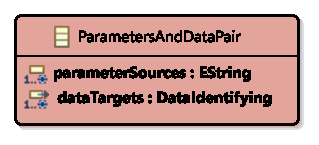
\includegraphics[width=0.19\textwidth]{images/old/repository.pdf}
	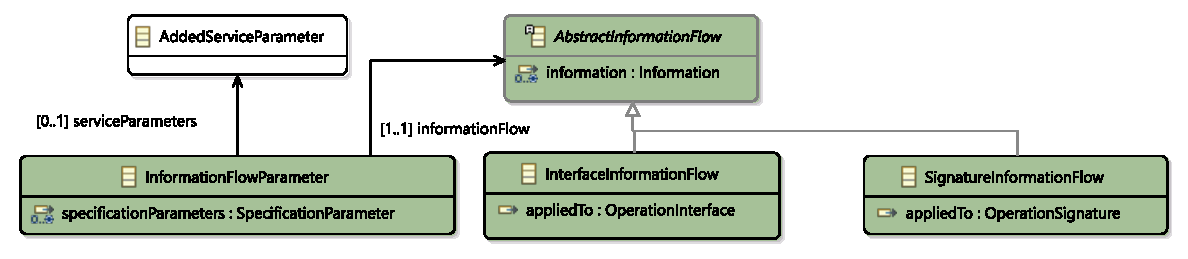
\includegraphics[width=0.77\textwidth]{images/new/repository.pdf}
	\caption{Klassendiagramm des Pakets \model{Repository}. Die grün markierten Klassen wurden hinzugefügt, um die Stereotypen  \model{ServiceParameterAddition} und \model{InformationFlowParameter} zu ersetzen. Die rot markierte Klasse \model{ParamterAndDataPair} wurde aus dem ursprünglichen Modell entfernt. Ihre Funktionalität wird jetzt von dem Paket \model{Information} übernommen}\label{repositoryPackage}
\end{figure}
\begin{figure}
\centering
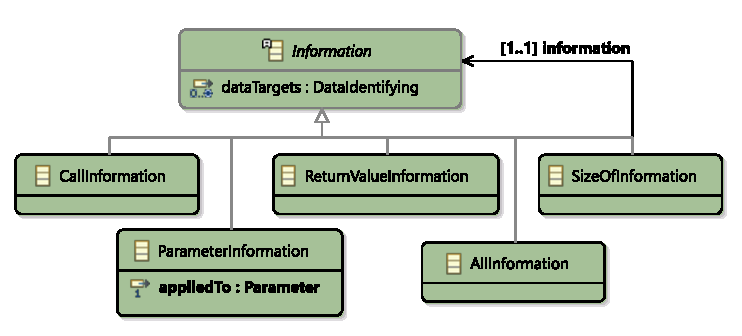
\includegraphics[width=\textwidth]{images/new/information.pdf}
\caption{Klassendiagramm des Pakets \model{Information}. Diese neu hinzugefügten Klassen übernehmen die Aufgabe der \model{ParamterAndDataPair} Klasse}\label{informationPackage}
\end{figure}
\begin{figure}	
	\centering
	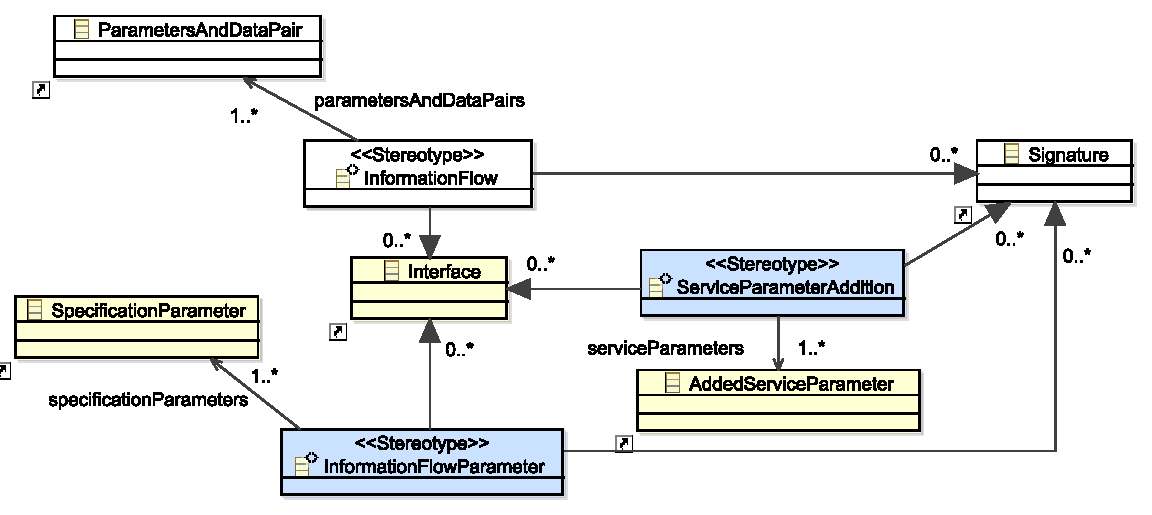
\includegraphics[width=\textwidth]{images/old/repositoryProfile.pdf}
	\caption{Teil des Confidentiality-Profils, welcher durch die neuen Klassen im Paket \model{Repository} ersetzt wird.}\label{repositoryProfil}
\end{figure}
\subsection{Resources}
Das Klassendiagramm des Pakets \model{Resources} ist zu sehen in \autoref{resoucresPackage}. Dieses Paket übernimmt im neuen Modell auch die Aufgaben der Stereotypen \model{Sharing}, \model{FutherPhysicalConnections}, \model{Encryption} und \model{LocationAndTamperProtection} (siehe \autoref{resoucresProfil}). Die Stereotypen \model{Sharing} und \model{FutherPhysicalConnections} wurden durch die Klasse \model{ResourceContainerConfidentiality} ersetzt. Der Stereotyp \model{Encryption} wird ersetzt durch die Klasse \model{Encryption}. Die Klasse \model{LocationsAndTemperProtectionsPair} wird zur abstrakten Klasse \model{AbstraktResourceProtection}, deren Unterklassen \model{LinkingResourceProtection} und \model{ResourceContainerProtection} referenzieren auf \model{LinkingResources} bzw. \model{ResourceContainer}, sodass der Stereotyp \model{LocationAndTamperProtection} nicht mehr benötigt wird. Allerdings kann eine \model{AbstraktResourceProtection} Instanz jetzt nur noch entweder auf \model{LinkingResoucres} oder auf \model{ResourceContainer} verweisen nicht mehr auf beides gleichzeitig. Wird dies benötigt, müssen dann jeweils eine \model{LinkingResourceProtection} und eine \model{ResourceContainerProtection} Instanz erstellt werden, die auf die gleichen \model{Locations} und \model{TamperProtections} zeigen.
\begin{figure}
	\centering
	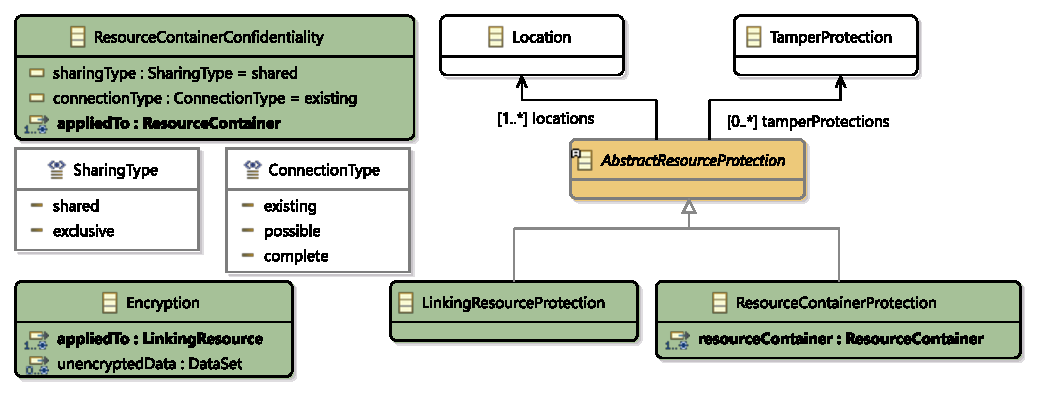
\includegraphics[width=\textwidth]{images/new/resources.pdf}
	\caption{Klassendiagramm des Pakets \model{Resources}. Die grün markierten Klassen sind neu erstelle Klassen, um die Funktionalität der Stereotypen in \autoref{resoucresProfil} zu übernehmen. Die gelb markierte Klasse \model{AbstractResourceProtection} ist die frühere \model{LocationAndTamperProtectionsPair} Klasse. Diese wurde lediglich umbenannt und zu einer abstrakten Klasse umgewandelt. }\label{resoucresPackage}
\end{figure}
\begin{figure}
	\centering
	\includegraphics[width=\textwidth]{images/old/resourceProfile.pdf}
	\caption{Teil des Confidentiality-Profils, welcher durch die neuen Klassen im Paket \model{Resources} ersetzt wird. }\label{resoucresProfil}
\end{figure}

\subsection{Adversary}
Das Paket \model{Adversary} (siehe \autoref{adversaryPackage}) hat sich nur dadurch verändert, dass nur die Referenz \model{mayTamperWith} nicht mehr auf die Klasse \model{LocationAndTamperProtectionsPair} zeigt, sondern auf die Klasse \model{AbstractResourceProtection}.
\begin{figure}[htbp]
	\centering
	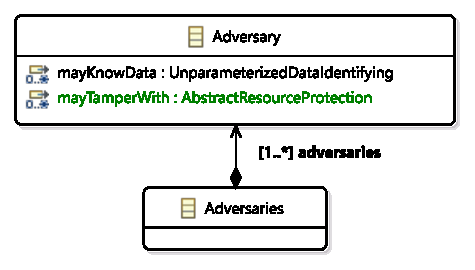
\includegraphics[width=0.6\textwidth]{images/new/adversary.pdf}
	\caption{Klassendiagramm des Pakets \model{Adversary}. Die Referenz zu der Klasse \model{AbstractResourceProtection} wurde geändert, da die Klasse umbenannt wurde.}\label{adversaryPackage}
\end{figure}

\section{PCM2Prolog Generator}
Der PCM2Prolog Generator wandelt Instanzen des Confidentiality-Modells in Prolog Prädikate um. Dieser musste im Rahmen dieses Praktikums so angepasst werden, dass trotz des veränderten Modells der Prolog Code identisch ist. Der Generator verwendet die Reflective-API von ECore und ist in Xtend geschrieben. Für jedes Entität wird die Methode \code{String generateDeeply(EObject e)} aufgerufen. Diese generiert für jedes Objekt und dessen Kinder Prolog Prädikate der Form: \code{referenceName(''objId'', [''refObjId1'',''refObjId2''])} für alle Referenzen und Attribute. In der Klasse \code{PCM2PrologXSBFilter} kann angegeben werden welche Klassen und Referenzen berücksichtigt werden sollen. Für Objekte, die nicht automatisch generiert werden können, können Dispatch-Methoden für die  \texttt{String generateDeeply(EObject e)} Methode definiert werden. Dies wurde für viele der neu hinzugefügten Klassen gemacht, um sicherzustellen, dass die Prolog Prädikate identisch zum ursprünglichen Modell sind.

Durch das Entfernen des Profil-Mechanismus hat sich die Richtung der Referenzen der PCM Komponenten zu den Modell Klassen umgedreht. Im ursprünglichen Modell hat ein Stereotyp PCM Klassen erweitert und hatte Referenzen auf Modell Klassen. Ein solcher Stereotyp wurde in ein einziges Prädikat pro PCM Objekt umgewandelt. Im neuen Modell gibt es allerdings für jeden früheren Stereotyp eine Modell Klasse die Referenzen auf ein oder mehrere PCM Objekte hat. Damit diese Referenzen trotzdem in ein Prädikat pro ResourceContainer umgesetzt werden können, werden die Referenzen in einer Map gespeichert wobei das PCM Objekt als Key dient. So kann nach dem alle Objekte verarbeitet wurden, für jedes PCM Objekt der Map ein Prädikat generiert werden mit den entsprechenden Referenzen zu den zugehörigen Modell Klassen.

\section{Evaluierung}
In dem Repository \code{Examples4SCBS} \cite{Examples4SCBS} werden eine Reihe an Beispiel Projekten für die Vertraulichkeitsanalyse zur Verfügung gestellt.Um zu überprüfen, ob der generierte Prolog Code identisch zu dem Prolog Code vor der Refaktorisierung ist, wurden die Beispiel Projekte \code{cloudscenario-minimized} und \code{iflowexample} im neuen Modell modelliert und das Ergebnis mit dem Ergebnis des ursprünglichen Modells verglichen. Diese zwei Beispiel Projekte wurden gewählt, da sie gemeinsam nahe zu alle Elemente des Confidentiality-Modells abdecken. Die einzige nicht verwendet Klasse ist die \model{SpecificationParameter2DataSetAssignment} Klasse. Diese wurde gesondert manuell getestet.

Um den Prolog Code automatisch vergleichbar zu machen, müssen beim Modellieren dieselben Identifier verwendet werden wie im original Projekt. Die Identifier der \model{LocationAndTemperProtectionsPair} Elemente müssen identisch zu den Identifierer der \model{AbstractResourceProtection} Elemente sein. Die Identifier der \model{ParameterAndDataPair} Elemente müssen identisch zu den Identifiern der \model{Information} Elemente sein. Die Identifier der anderen neuen Klassen können frei gewählt werden.

Beim Generieren des Prolog Codes müssen die Optionen fullIDs, singleFile und noComment ausgewählt werden, da bewusst die Kommentare nicht identisch sind, sondern so gewählt, dass auf die Entitäten, aus denen die Prolog Prädikate generiert wurden, zurück geschlossen werden kann. Im letzten Schritt müssen die Ausgabe Dateien noch vereinheitlicht werden. Dies ist lediglich notwendig um die die Dateien automatisch vergleichen zu können. Es gibt viele Prädikate der Form: \code{prädikatName(''entity'',[''child1'',''child1'',''child3'']).} Die Reihenfolge der Elemente \code{child1} bis \code{child3} in der Liste hat keine Auswirkungen auf die Berechnung. Deshalb werden die Listenelemente solcher Prädikate alphabetisch sortiert. Außerdem kann sich die Reihenfolge der Zeilen unterscheiden, je nach dem in welcher Reihenfolge die Objekte verarbeitet wurden. Deshalb wird anschließend die Datei zeilenweise sortiert und leere Zeilen entfernt. Diese beiden Schritte können mit einem einfachen Shell Skript durchgeführt werden. Auf den vereinheitlichen Dateien kann dann der \code{diff} Befehl der GNU Diffutils ausgeführt werden.

Beide Beispiel Projekte \code{CloudScenario-minimized} und \code{IflowExample} konnten erfolgreich so im neuen Modell modelliert werden, dass der Prolog Code identisch ist. Allerdings hatten beide Projekte undefinierte Referenzen die zu zufälligen Identifiern in Prädikaten führen. Diese musste erst entfernt werden bevor der Vergleich durchgeführt werden konnte. Im \code{cloudscenario-minimized} Beispiel gab es eine Referenz  in der \code{cloud.adverary} Datei auf ein \model{LocationAndTemperProtectionsPair}, welches nicht in der \code{cloud.confidentielity} Datei definiert war. Im \code{iflowexample} gab es  undefinierte Referenzen innerhalb der Elementen \code{Allocation Energy Visualization}, \code{Allocation Database DBMS} und \code{Allocation Energy Meter} im File \code{default.allocation} und innerhalb der Elemente \code{ProvDelegation Provided AnInterface -> Provided AnInterface AComponent}, \code{Connector Energy Visualization -> Database} und \code{Connector Energy Visualization -> Energy Meter Assembly Context} und in der \code{default.system} Datei. Da diese Elemente nicht in der Confidentiality-Instanz referenziert werden, konnten diese gelöscht werden.

\section{Fazit}
Die Refaktorisierung der Vertraulichkeitsanalyse wurde vorgenommen, da es im ursprüngliche Modell implizite Referenzen im Hilfe von String Attributen gab und der Profil-Mechanismus in Kombination mit Eclipse in der Vergangenheit Probleme verursacht hat. Ersteres wurde durch die Modellierung als explizite Referenzen und eigene Klassen gelöst, letzteres durch Einführen von neuen Klassen oder Erweitern von besehenden Klassen die Referenzen auf PCM Klassen haben. Außerdem musste der \code{PCM2Prolog} Generator angepasst werden, damit trotz der Änderungen am Modell der generiere Prolog Code gleich bleibt. Das konnte erreicht werden mit der Ausnahme von Wiederverwendung von Hilfsklassen wie zum Beispiel der Klasse \model{ParameterAndDataPair} oder \model{LocationAndTemperProtectionsPair}. In diesen Fällen kann der gleiche Sachverhalt aber auch durch mehrere dieser Klassen mit gleichen Parametern modelliert werden, deshalb ist es in diesen Fällen vertretbar, dass für diese Instanzen der Prolog Code nicht identisch ist.
%% --------------------
%% |   Bibliography   |
%% --------------------

%% Add entry to the table of contents for the bibliography
%\printbibliography[heading=bibintoc]
\printbibliography

\end{document}